\documentclass{report}
\usepackage{graphicx}
\usepackage[round]{natbib}
%\usepackage[backend=biber]{biblatex}
%\addbibresource{bib.bib} % with extension


\begin{document}

\author{Hamid Shayestehmanesh}
\title{Creating a instrument based on movements in webcam view}
\maketitle
\tableofcontents
\newpage

\section{Main Project Idea}

The main idea in this project is to build a HCI application which can shape the music and users can draw it. In other words, we want to design and build an application which is able to translate hands movements to meaningful sounds and build a new electronic music instrument.
\subsection{More Specified}
In this project we are following the goal to design an architecture of such program and building a prototype. To detect hands and their movements we use different colored cameras and regular speakers are used to generate sounds. Devices and implementation environment will be discussed in details later.
\pagebreak


\section{Literature}
This section is the most important section in this report. All next parts are based on information explained in this chapter. This section tries to translate needed knowledge of music from musician language to computer scientists language thus they can use the information to build different applications related to music.
\subsection{Music Language and Important Information}
Any one of the systems of signs and words that are used by a particular group of people to communicate and transfer knowledge about a specific subject is called a language\citep{Lang}. Nowadays, translation has become very common but, it faces different difficulties. Finding the best word in destination language, demonstrating emotions, feelings and, keeping the structure of the article are some of the hardest problems of translating. Here, we are trying to translate language of a musician to engineering language. So, we will explain different important aspect of musical notes which are mandatory to know about while building a new instrument. To reach our goal we explain what is note language and state it in engineering form to find out what is important to write a music. 

\subsubsection{Note Language}
Note language like other languages contains some sign which works as it's letters and they are written in lines. Human languages are usually written in a line with one lane however, note language has 5 lanes and they are very important. Each note has an actual sound, a length of time and power(bolandi seda). 
\begin{itemize}
\item[Octave: ]{Octave of a note is determined by its place on the lanes. It's determined by the start place and end place of the note vertically. For example in figure x first note starts in lane 3 and ends in lane 5. }
\item[Note: ]{Notes are determined as the same as octave. Actually the vertical place shows note and octave together.}
\item[Octave and Note: ]{Octave and Note are used together to find out the exact frequency that the music should be played in. }
\item[Length of Time: ]{In the note language length of time is handle with the shape of a  note. Any article in note language has a base time and each note means a ratio over the base time. For example, note \textbf{XXX figure folan!} is $1/2$ of base time. If the base time of a music is 10ms then this note means 5ms therefore, the player will played a frequency specified by the place of the note for 5ms.}
\end{itemize}
However with knowing time and frequency of each note this is possible to write a meaningful song but there's some more basic operators which can make a simple music to famous magical one.
\begin{itemize}
\item[Additional signs  on top of the notes: ]{Except the frequency and length of a note we should also determine how loud should it be played. Looking deep in music we can find this is meaningless to give each note a number or sign to demonstrate the loudness value. This would make the language very complex and also we should define loudness with measurable variable which is actually hard to understand for a musician. Musician mostly decides by intuition thus, they don't like counting! The language notify the player to play louder or more quite and also it shows where is the pick and how loud the pick is. In engineering aspect it may seem very obvious what to do when jumping to next note. You subtract your measure of current loudness from the pick and then divide it by the number of jumps but, it is not that simple in reality. As mentioned we are trying to design and implement a prototype so the obvious idea would be sufficient for now. }
\end{itemize} 
Talking about loudness this should be mentioned that loudness is different to harshness. When we make a music louder the frequency and length and the feeling doesn't change but when we make a music harsher we exactly change the way it is. For example, compare the song "Maste Cheshat" by Ebrahim Hamedi sang in 1379 with the same song by E. Hamedi sang in 1394. Same song, same lyrics, same singer but the harshness is very different. You may dance tango with first one but use the second one in disco! In a better word the feeling of the music can change it completely. Again, we skip the feeling and keep with the three basic principles mentioned.\newline
Addition to frequency, length and loudness of a note many other things can be gain from note language like Bemol, Diez or Dot. We will omit more information of the language as they actually give advance data about these three principles or how to acrobat between them. They will complicate our report however it may have no gain for us.


\iffalse
octave : ja nesbat be khootoot
note : ja nesbat be khootoot
time : shekl, nesbat be time avalie - agar noghte dasht mishe 1.5 barabar
frequency : octave and note
fasele hashoon : sefr hast
diez (nim parde bala) :
bemol (nim parde paeen) : 
agar ba khat beham vasl shodam vasleshoon mikone va note ro kamel tamoom nemikoni baddi ro shoro mikoni
agar nadasht ye chos mesghali fasele dare!
bolandi seda : ye seri shekl roie sareshoon
takid : bazam shekl roosh


meta data:
	speed = 250 masalan hast, ke clock ba estefade az metronom moshakhas mishe.

just this!
anything else Sara ?
\fi


\subsection{Meta Data}
Each music written in note language has some meta data. This meta data includes the speed of the song or in other words how long should a note with one unit of time takes. What should the feeling of the musician be? A few other information exists but they have no important affect on our architecture. 


\subsection{Conclusion}
To conclude from an engineer approach, to play a song we need to know frequency and loudness of the song and also this have some different ways to move from a frequency and loudness to another frequency and loudness. It must be able to move fast or slowly. 



\section{Architecture}



\pagebreak
\section{Implementation}
During this section, first prototype is discussed, then we will discuss one advanced input. 



\subsection{Prototype}

\subsubsection{Abstract}{A minimal model is implemented using Python, OpenCV(Tracking the Object) and Pygame(Generating Sounds). In this model there is an element detected by camera which frequency and amplitude is computed base on its coordinates. Coordination of the element identifies by color segmentation.}

\iffalse
Vertically changes the frequency of sound and moving it horizontally changes sounds' amplitude


complete the prototype part and 

\fi

\subsubsection{Prototype}
The prototype works with one specific element. The idea is to determine the place of the element and use the coordination for the rest of the application. To find the element coordinates, we use color segmentation, in other word, we convert every pixel to black except those have the specified color. Filtering the color or color segmentation will give us a black and white frame which everything should be black but the element due to the fact that it is built in the specified color. In practice some other small areas will be converted to white. \textbf{figure folan! noise!} To solve this problem we add a noise reduction after getting the black and white image. \textit{Eroding} and \textit{Dilating} the image will fairly solve the noise problem. Eroding will :: . Dilating will :::. By performing Erode and Dilate functions continuthe small white pieces will be removed \textit{figure folan!}. It will also remove around the element part which may turn it to a few parts. Dilating is used to merge the main white unit if it's affected by the Erode function. In next step we should identify the element by one point to track it's movements. To detect the center of element, first draw a contour around each white color region. As a contour won't usually have a good shape, find the minimum circle around the contour to have a presentation of the element coordination in frame. Choose the biggest circle if there is more than one contour. Also the center of circle is a good one-point identifier. \newline
Next, by comparing two last center of this imaginary circle can help us detect any movement of the element. Now that we have coordination and movement, we can update our frequency and amplitude. Generate and play a sound with specified frequency and amplitude using Pygame. Moving vertically change the frequency of sound and moving it horizontally changes sounds' amplitude.  \newline

\subsection{Object Tracking}
As mentioned we need to detect and follow an object in camera streams. In this section we will demonstrate how and why the object is evolved. We will discuss each element one by one and explain their flaws.

\subsubsection{Try 1}
The first two Objects are recognized by their size and color in frames. The problem with these two objects is that if any object with the same color appears in the frame and has an appropriate size, the system may follow the wrong object. So the system is not robust. \newline
\begin{center}
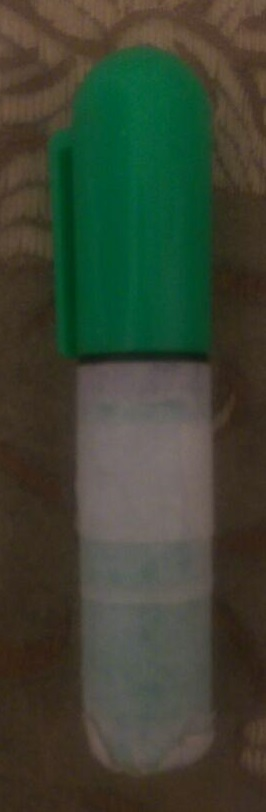
\includegraphics[width=1in]{Object1.jpg}
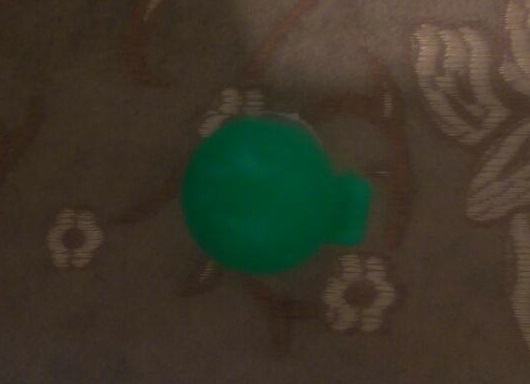
\includegraphics[width=3in]{Object1-2.jpg}\newline \figurename{Object1} Used from top (second image)	
\end{center}
\subsubsection{Try 2}
One easy idea to solve the problem is to increase the size of the object. This way 
\begin{center}
	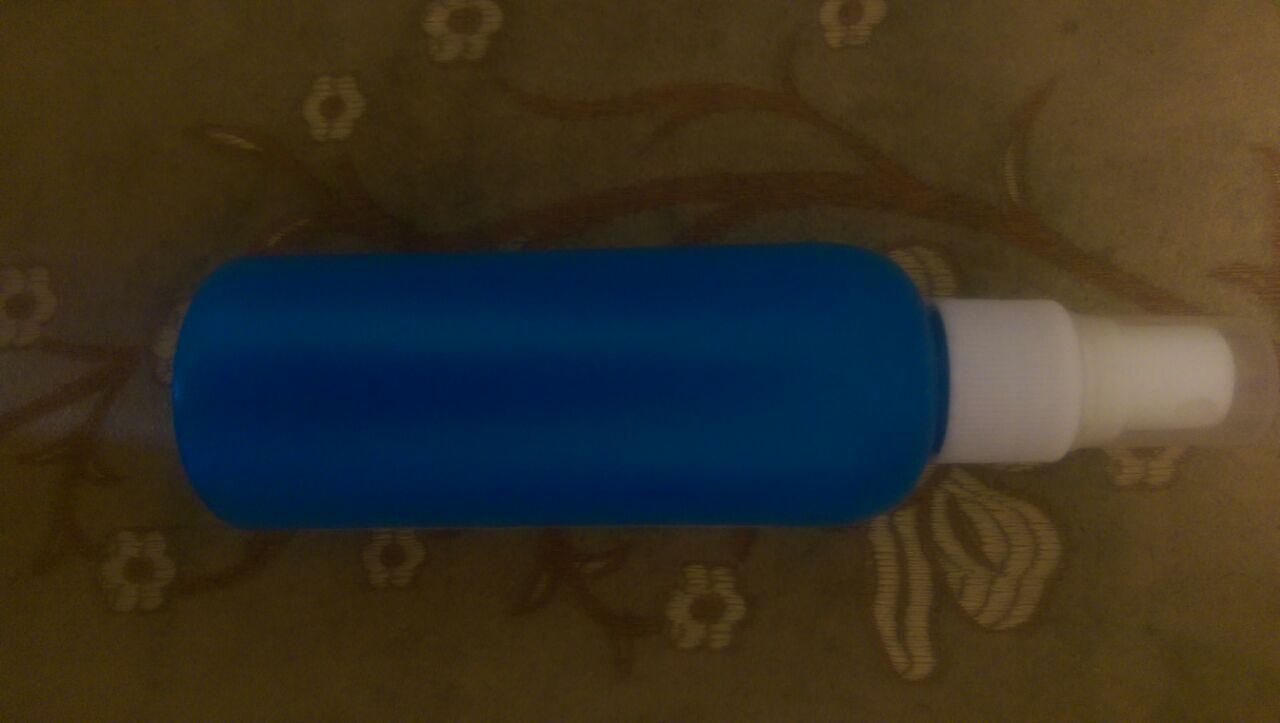
\includegraphics[width=3in]{Object2.jpg} \newline \figurename{Object2} Used from side 
\end{center}
Due to the fact that this step still recognize the object by size and color increasing the size won't help, mostly because of noises, sometimes the contour around the detected color becomes small specially in fast pace movements. Also increasing the size of the object has two consequences, first due to big size of the contour around the detected object it cannot move upon one direction much. It's shorter than what it should be. A little noise can change the center's coordination too much and make the system very vulnerable to noise. Another point is that an element with this size is far from practical. 
\subsubsection{Try 3}
In next attempt we need to resize the element and 
One Idea to solve the problem is to create a specific background, therefore the colored point won't be lost in the background color. First attempt with this idea is one stick on hand. \newline
\begin{center}
	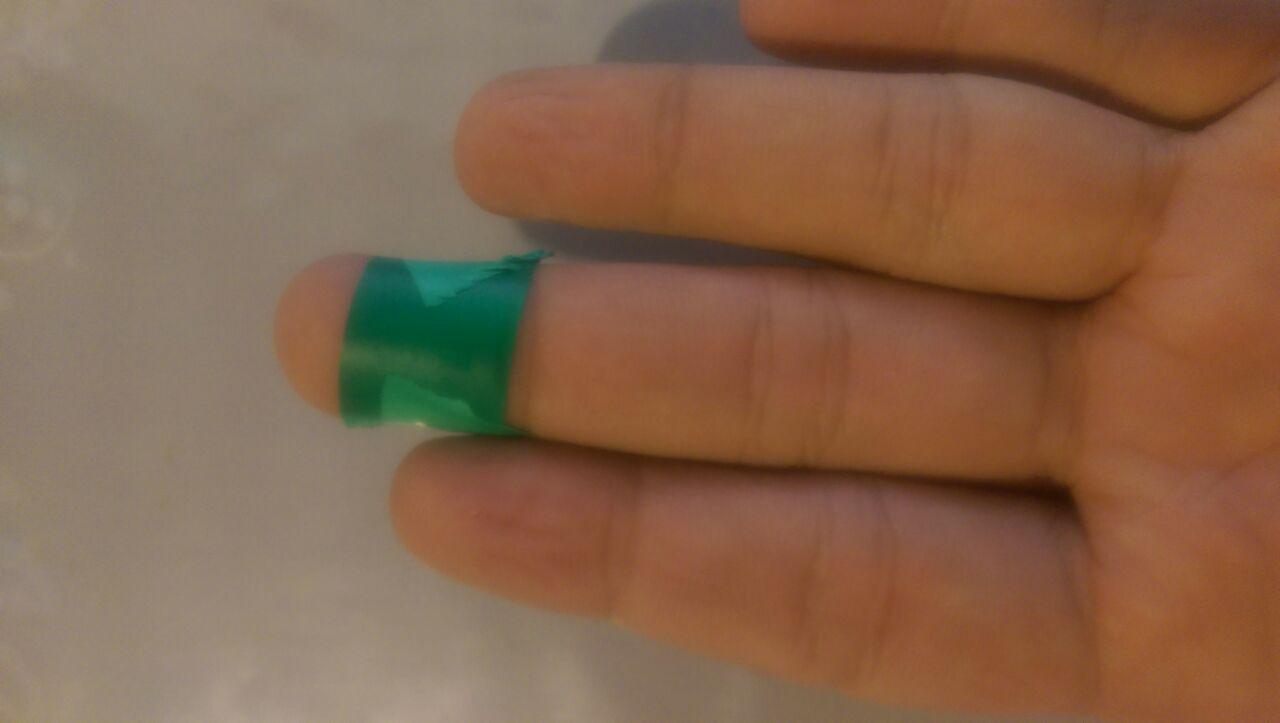
\includegraphics[width=3in]{Object3.jpg}\newline \figurename{The green color was seperated to detect the point}
\end{center}
\subsubsection{Try 4}
Even though a green stick on the finger seems detectable but in practice the color of skin is not very stable so it isn't very helpful as a background, also in light has a enormous effect on the color.
\subsubsection{Try 5}
To solve the problem some red stick are added in up and down and then on left and right. Even the system works fine with only  up and down red sticks but adding left and right ones will help the system when very bright lights exists in the frame.
\begin{center}
	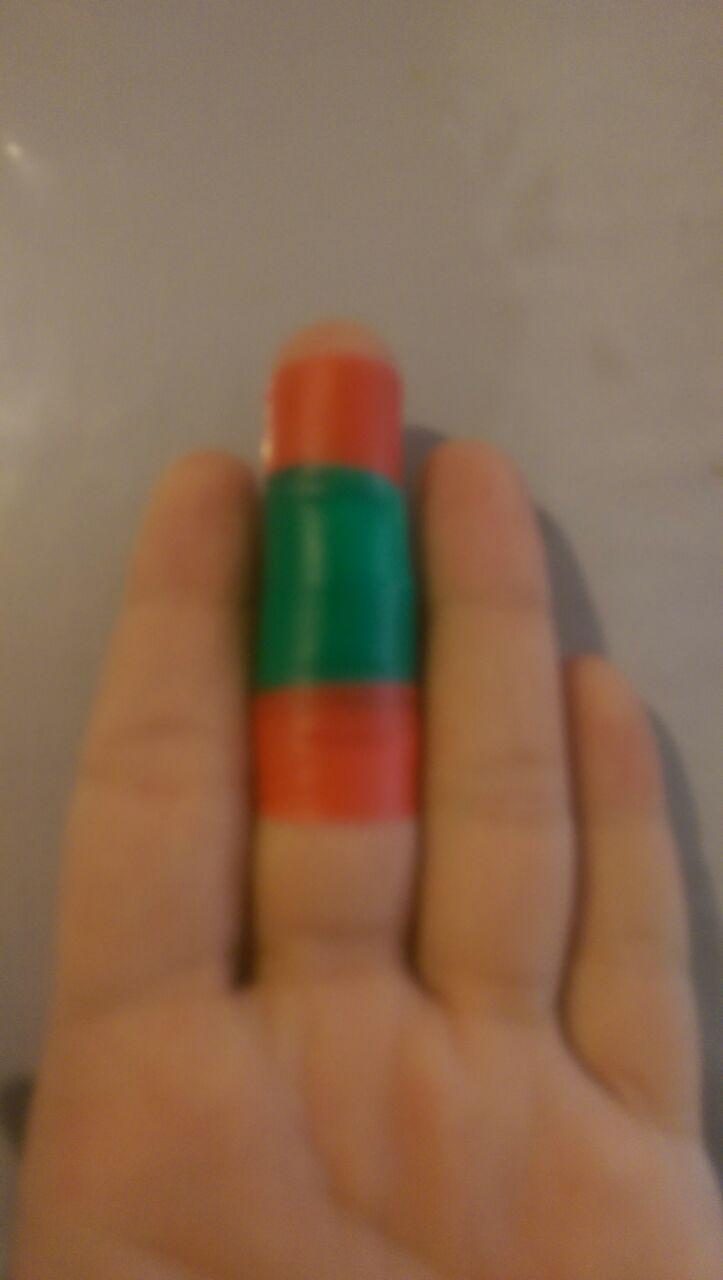
\includegraphics[width=2in]{Object4.jpg}
	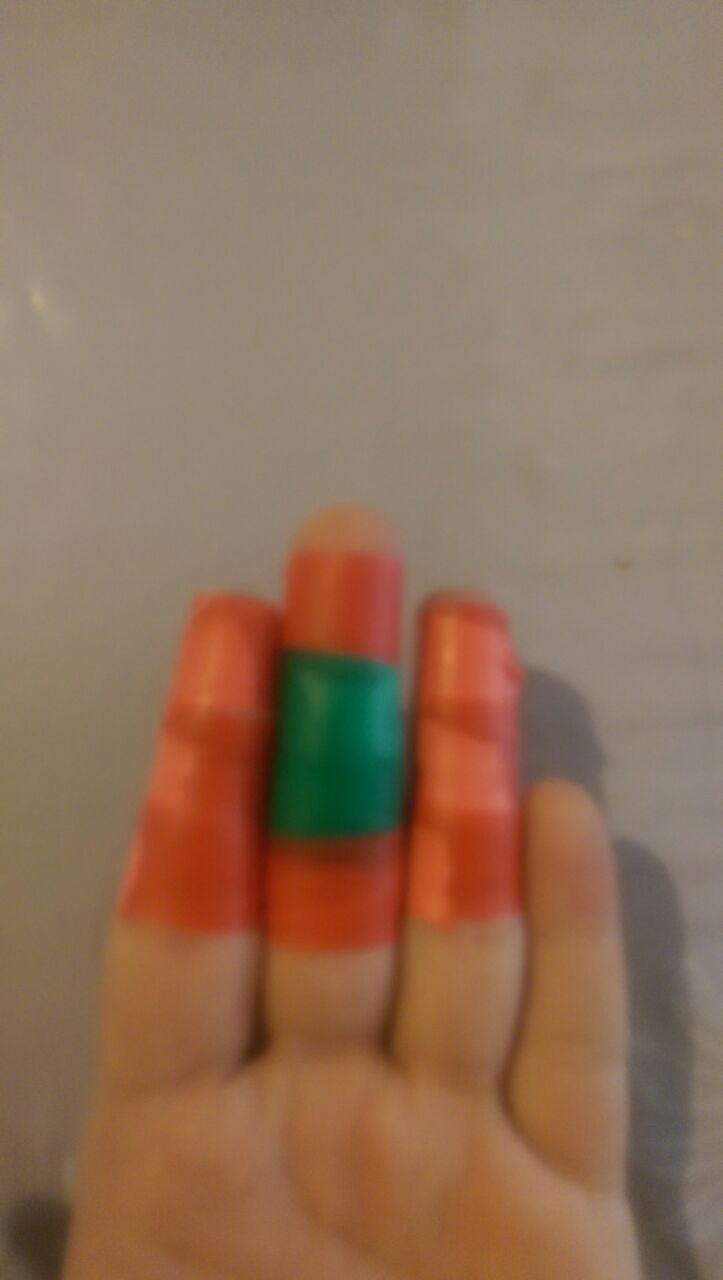
\includegraphics[width=2in]{Object5.jpg}
\end{center}
Due to the fact that sticks are very annoying I created something with papers.
\begin{center}
	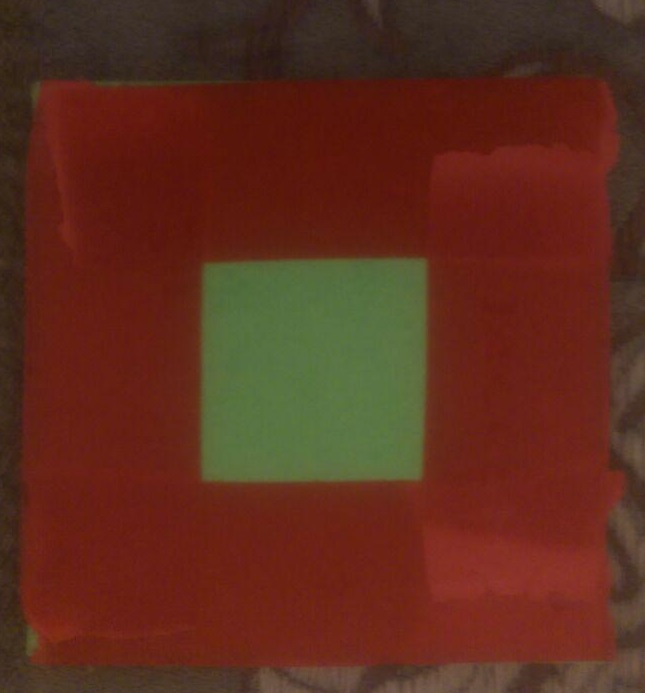
\includegraphics[width=2in]{Object6.jpg} \newline
	\figurename{Created with papers}
\end{center}

\subsubsection{Try 6}
The papered object worked fine but because of the small background sometimes following the point became hard. To solve the problem we use the fact that one's hand won't move very fast, so if call current position of point $p_1 = (x_1, y_1)$ and next position $p_2 = (x_2, y_2)$ then the distance between $p_1, p_2$ is less than $C$. So if we know the place of point, so we don't have to search the hole next frame to find the point. We have to search only a part of it, so a square with upper left point of $p_1 - (C, C)$ and the lower right point of $p_1 + (C, C)$ 
\subsubsection{Try 7}
If we could ever make the background bigger the system could work more robust. We created a glove with the point one it. The big background it used to create help the system to track the point using only mentioned square. 
\begin{center}
	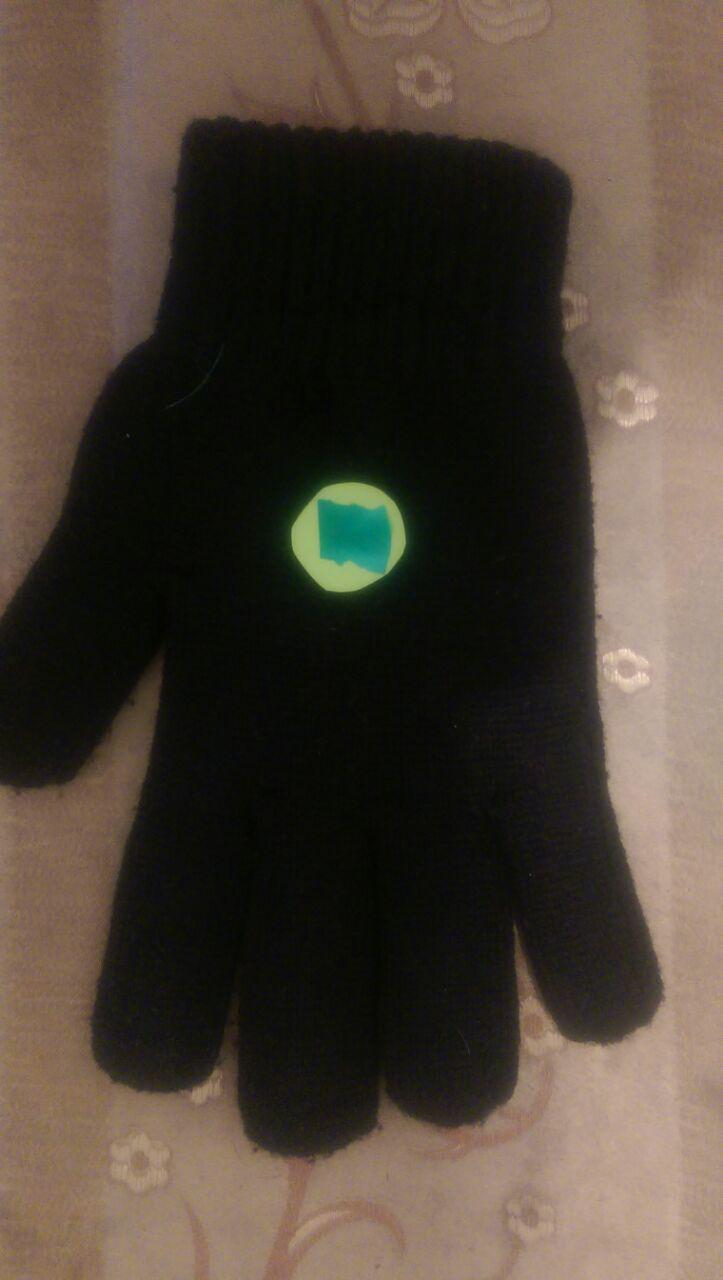
\includegraphics[width=3in]{Object7.jpg}
\end{center}
This object works very well but yet light can make huge distractions. To solve the problem we change many different color for the glove ( as the background ) (Colors are shown below) and the Red Dark seemed to work better than others. 
\begin{center}
	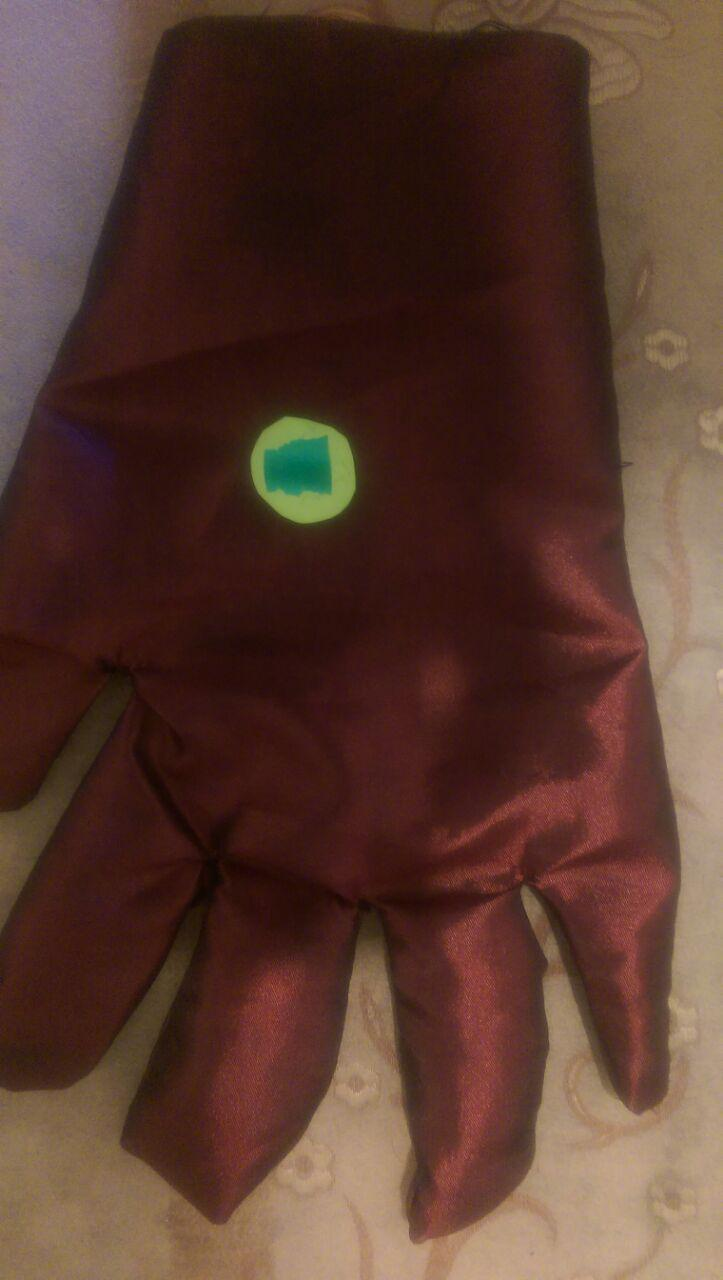
\includegraphics[width=3in]{Object8.jpg}
\end{center}

\section{Playing Notes}
To play notes we break the frame into 9 parts, one for silence and 8 others for 8 different notes. Shown below.

\section{OpenCV}

\section{Future Work}
It can be implemented on Android or any other mobile frameworks.
\section{Other Technologies}
A programming language called Chuck has been created in Princeton university. ChucK is a programming language for real-time sound synthesis and music creation. The problem with this language is that it's doesn't support any library which can use webcam or any type of camera, neither easy way to connect it to another programming language.
\bibliographystyle{plainnat}
\bibliography{bibfile}

\end{document}